\documentclass[11pt,aspectratio=169]{beamer}
\usetheme{Madrid}

% ======================= PACKAGES =======================
\usepackage{graphicx}
\usepackage{booktabs}
\usepackage{adjustbox}
\usepackage{multicol}
\usepackage{amsmath}
\usepackage{amssymb}
\usepackage{tikz}
\usetikzlibrary{arrows,shapes,positioning,shadows,trees}
\usepackage{listings}
\usepackage{xcolor}

% ======================= COLOR DEFINITIONS =======================
% Primary color scheme: Blue/Teal for Digital Finance
\definecolor{dfblue}{RGB}{0,102,204}
\definecolor{dfteal}{RGB}{0,153,153}
\definecolor{dfcyan}{RGB}{51,187,204}
\definecolor{dflightblue}{RGB}{153,204,255}
\definecolor{dflightblue2}{RGB}{173,214,255}
\definecolor{dflightblue3}{RGB}{193,224,255}
\definecolor{dflightblue4}{RGB}{213,234,255}

% Accent colors for finance applications
\definecolor{dfgreen}{RGB}{44, 160, 44}
\definecolor{dfred}{RGB}{214, 39, 40}
\definecolor{dforange}{RGB}{255, 127, 14}
\definecolor{dfgray}{RGB}{127, 127, 127}

% Utility colors
\definecolor{lightgray}{RGB}{240, 240, 240}
\definecolor{midgray}{RGB}{180, 180, 180}
\definecolor{codebg}{RGB}{245, 245, 245}

% ======================= THEME CUSTOMIZATION =======================
% Apply Digital Finance color scheme to Madrid theme
\setbeamercolor{palette primary}{bg=dflightblue3,fg=dfblue}
\setbeamercolor{palette secondary}{bg=dflightblue2,fg=dfblue}
\setbeamercolor{palette tertiary}{bg=dfteal,fg=white}
\setbeamercolor{palette quaternary}{bg=dfblue,fg=white}

\setbeamercolor{structure}{fg=dfblue}
\setbeamercolor{section in toc}{fg=dfblue}
\setbeamercolor{subsection in toc}{fg=dfteal}
\setbeamercolor{title}{fg=dfblue}
\setbeamercolor{frametitle}{fg=dfblue,bg=dflightblue3}
\setbeamercolor{block title}{bg=dflightblue2,fg=dfblue}
\setbeamercolor{block body}{bg=dflightblue4,fg=black}

% Remove navigation symbols for cleaner look
\setbeamertemplate{navigation symbols}{}

% Clean itemize/enumerate
\setbeamertemplate{itemize items}[circle]
\setbeamertemplate{enumerate items}[default]

% Margins for readability
\setbeamersize{text margin left=8mm,text margin right=8mm}

% ======================= LISTINGS CONFIGURATION =======================
% Python code style
\lstdefinestyle{pythonstyle}{
    language=Python,
    basicstyle=\ttfamily\footnotesize,
    keywordstyle=\color{dfblue}\bfseries,
    stringstyle=\color{dforange},
    commentstyle=\color{dfgray}\itshape,
    numberstyle=\tiny\color{dfgray},
    numbers=left,
    numbersep=5pt,
    backgroundcolor=\color{codebg},
    showspaces=false,
    showstringspaces=false,
    showtabs=false,
    frame=single,
    rulecolor=\color{midgray},
    tabsize=4,
    captionpos=b,
    breaklines=true,
    breakatwhitespace=false,
    escapeinside={(*@}{@*)},
    xleftmargin=10pt,
    xrightmargin=10pt
}

% Solidity code style
\lstdefinestyle{soliditystyle}{
    language=Java, % closest approximation
    basicstyle=\ttfamily\footnotesize,
    keywordstyle=\color{dfteal}\bfseries,
    stringstyle=\color{dforange},
    commentstyle=\color{dfgray}\itshape,
    numberstyle=\tiny\color{dfgray},
    numbers=left,
    numbersep=5pt,
    backgroundcolor=\color{codebg},
    showspaces=false,
    showstringspaces=false,
    showtabs=false,
    frame=single,
    rulecolor=\color{midgray},
    tabsize=2,
    captionpos=b,
    breaklines=true,
    breakatwhitespace=false,
    escapeinside={(*@}{@*)},
    xleftmargin=10pt,
    xrightmargin=10pt,
    morekeywords={pragma, contract, function, returns, public, private, view, pure, payable, address, uint256, mapping, event, modifier}
}

% Inline code command
\newcommand{\code}[1]{\texttt{\color{dfblue}#1}}

% ======================= CUSTOM COMMANDS =======================
% Bottom annotation (Madrid-style)
\newcommand{\bottomnote}[1]{%
\vfill
\vspace{-2mm}
\textcolor{dflightblue2}{\rule{\textwidth}{0.4pt}}
\vspace{1mm}
\footnotesize
\textbf{#1}
}

% Compact list spacing
\newcommand{\compactlist}{%
\setlength{\itemsep}{0pt}%
\setlength{\parskip}{0pt}%
\setlength{\parsep}{0pt}%
}

% Chart placeholder
\newcommand{\chartplaceholder}[2][5cm]{%
\begin{center}
\begin{adjustbox}{max width=0.95\textwidth, max height=#1}
\framebox[\textwidth][c]{%
\rule{0pt}{#1}%
\textcolor{midgray}{[#2]}%
}
\end{adjustbox}
\end{center}
}

% ======================= FINANCE NOTATION MACROS =======================
% Probability and statistics
\newcommand{\E}{\mathbb{E}} % Expected value
\newcommand{\Var}{\mathrm{Var}} % Variance
\newcommand{\Cov}{\mathrm{Cov}} % Covariance
\newcommand{\Prob}{\mathbb{P}} % Probability

% Distributions
\newcommand{\Normal}{\mathcal{N}} % Normal distribution
\newcommand{\Uniform}{\mathcal{U}} % Uniform distribution

% Returns and prices
\newcommand{\Ret}{R} % Return
\newcommand{\LogRet}{r} % Log return
\newcommand{\Price}{S} % Price/Stock price
\newcommand{\Strike}{K} % Strike price

% Options and derivatives
\newcommand{\CallPrice}{C} % Call option price
\newcommand{\PutPrice}{P} % Put option price
\newcommand{\Greeks}[1]{\mathit{#1}} % Greek letters

% Risk measures
\newcommand{\VaR}{\mathrm{VaR}} % Value at Risk
\newcommand{\CVaR}{\mathrm{CVaR}} % Conditional VaR
\newcommand{\Sharpe}{\mathrm{SR}} % Sharpe Ratio

% Time series
\newcommand{\AR}{\mathrm{AR}} % Autoregressive
\newcommand{\MA}{\mathrm{MA}} % Moving average
\newcommand{\GARCH}{\mathrm{GARCH}} % GARCH

% Blockchain/Crypto
\newcommand{\Hash}{\mathrm{Hash}} % Hash function
\newcommand{\Block}{\mathcal{B}} % Block
\newcommand{\Chain}{\mathcal{C}} % Chain

% Real numbers, integers
\newcommand{\R}{\mathbb{R}}
\newcommand{\Z}{\mathbb{Z}}
\newcommand{\N}{\mathbb{N}}

% ======================= TIKZ STYLES =======================
% Styles for finance-related diagrams
\tikzstyle{process} = [rectangle, minimum width=3cm, minimum height=1cm, text centered, draw=dfblue, fill=dflightblue4, thick]
\tikzstyle{decision} = [diamond, minimum width=3cm, minimum height=1cm, text centered, draw=dfteal, fill=dflightblue4, thick]
\tikzstyle{arrow} = [thick,->,>=stealth,color=dfblue]
\tikzstyle{blockchain} = [rectangle, rounded corners, minimum width=2.5cm, minimum height=1cm, text centered, draw=dfteal, fill=dflightblue3, thick]
\tikzstyle{transaction} = [circle, minimum size=0.8cm, text centered, draw=dforange, fill=dflightblue4, thick]

% ======================= FOOTER TEMPLATE =======================
\setbeamertemplate{footline}{
    \hbox{\begin{beamercolorbox}[wd=\paperwidth,ht=2.5ex,dp=1ex,leftskip=.5em,rightskip=.5em]{author in head/foot}
    \tiny
    \textbf{Digital Finance} \hfill
    Joerg Osterrieder \hfill
    \insertdate \hfill
    Page \insertframenumber{} / \inserttotalframenumber
    \end{beamercolorbox}}
}

% ======================= SECTION DIVIDER TEMPLATE =======================
\AtBeginSection[]{
\begin{frame}[plain]
\vfill
\centering
\begin{beamercolorbox}[sep=12pt,center]{title}
\usebeamerfont{title}\LARGE\insertsection\par
\end{beamercolorbox}
\vfill
\end{frame}
}


\title{Topic 6.3: Building Your Digital Finance Worldview}
\subtitle{A Framework for Evaluating Innovation}
\author{Joerg Osterrieder}
\institute{Digital Finance}
\date{2025}

\begin{document}

% ---------------------------------------------------------------------
% Slide 1: Title slide
% ---------------------------------------------------------------------
\begin{frame}[plain]
\titlepage
\end{frame}

% ---------------------------------------------------------------------
% Slide 2: Learning Objectives
% ---------------------------------------------------------------------
\begin{frame}{Learning Objectives}
By the end of this topic, you will be able to:

\begin{enumerate}
\item \textbf{Apply} a systematic framework for evaluating digital finance innovations
\item \textbf{Distinguish} between rapidly changing facts and durable principles
\item \textbf{Analyze} innovations using the six-question Innovation Scorecard
\item \textbf{Identify} trade-offs inherent in any digital finance design choice
\item \textbf{Synthesize} technical, economic, regulatory, and social perspectives
\item \textbf{Develop} your own informed worldview for navigating digital finance
\end{enumerate}

\vspace{0.3cm}
\begin{block}{Goal}
Equip you with a \textbf{thinking framework} that remains useful for years, not facts that quickly become outdated.
\end{block}
\end{frame}

% ---------------------------------------------------------------------
% Slide 3: Prerequisites/Background
% ---------------------------------------------------------------------
\begin{frame}{Prerequisites: What You've Learned}
\begin{columns}[T]
\begin{column}{0.48\textwidth}
\textbf{Days 1-3 Foundation:}
\begin{itemize}
\item Nature of money and trust
\item Financial system pain points
\item FinTech vs. Crypto/DeFi distinctions
\item Digital payments and APIs
\item Platform economics
\item Cryptographic foundations
\item Blockchain mechanics
\end{itemize}
\end{column}
\begin{column}{0.48\textwidth}
\textbf{Days 4-6 Applications:}
\begin{itemize}
\item Smart contracts
\item DeFi primitives and stablecoins
\item Tokenization and CBDCs
\item What goes wrong (failures)
\item Regulatory landscapes
\item Privacy and inclusion
\item AI in digital finance
\end{itemize}
\end{column}
\end{columns}

\vspace{0.3cm}
\begin{alertblock}{Integration Challenge}
Today we \textbf{integrate} all these perspectives into a coherent analytical framework.
\end{alertblock}
\end{frame}

% ---------------------------------------------------------------------
% Slide 4: The Challenge of Permanent Knowledge
% ---------------------------------------------------------------------
\begin{frame}{The Challenge of Permanent Knowledge}
\begin{columns}[T]
\begin{column}{0.48\textwidth}
\textbf{What Changes Rapidly:}
\begin{itemize}
\item Specific protocols and platforms
\item Token prices and market caps
\item Regulatory stance by jurisdiction
\item Leading companies and projects
\item Technical implementation details
\end{itemize}
\end{column}
\begin{column}{0.48\textwidth}
\textbf{What's More Durable:}
\begin{itemize}
\item Economic first principles
\item Security vs. convenience tradeoffs
\item Decentralization spectrum
\item Regulatory logic and goals
\item Human behavior patterns
\end{itemize}
\end{column}
\end{columns}

\vspace{0.5cm}
\begin{block}{Our Approach}
Give you a \textbf{framework}---not facts that will become outdated, but a way of thinking that remains useful for years.
\end{block}
\end{frame}

% ---------------------------------------------------------------------
% Slide 5: The Digital Finance Innovation Scorecard
% ---------------------------------------------------------------------
\begin{frame}{The Digital Finance Innovation Scorecard}
\begin{center}
\textbf{Six Questions for Any Digital Finance Innovation}
\end{center}

\begin{enumerate}
\item \textbf{PROBLEM}: What real problem does this solve, and for whom?
\item \textbf{MECHANISM}: How does it actually work (technically and economically)?
\item \textbf{TRADEOFFS}: What are the key tradeoffs and design choices?
\item \textbf{RISKS}: What could go wrong (technical, economic, regulatory)?
\item \textbf{REGULATORY STATUS}: Where does it fit in the regulatory landscape?
\item \textbf{WHO BENEFITS}: Who captures value, and who bears costs?
\end{enumerate}

\vspace{0.3cm}
\begin{exampleblock}{Design Principle}
These questions work whether you're evaluating Bitcoin in 2009, DeFi in 2020, or whatever comes next in 2030.
\end{exampleblock}
\end{frame}

% ---------------------------------------------------------------------
% Slide 6: Question 1 - PROBLEM
% ---------------------------------------------------------------------
\begin{frame}{Question 1: PROBLEM}
\begin{block}{Key Sub-Questions}
\begin{itemize}
\item What existing pain point does this address?
\item Who has this problem? (Individuals, businesses, institutions?)
\item How big is the problem? (Market size, frequency, severity)
\item How is it solved today, and why is that solution inadequate?
\item Is the problem real, or is this a ``solution looking for a problem''?
\end{itemize}
\end{block}

\vspace{0.3cm}
\textbf{Red Flags:}
\begin{itemize}
\item Vague problem statements (``revolutionize finance'')
\item No clear user with an urgent need
\item The problem is already well-solved by existing technology
\item Solving a problem only crypto enthusiasts have
\end{itemize}
\end{frame}

% ---------------------------------------------------------------------
% Slide 7: Problem Analysis Examples
% ---------------------------------------------------------------------
\begin{frame}{Problem Analysis: Real-World Examples}
\begin{table}[h]
\centering
\footnotesize
\begin{tabular}{p{2.5cm}p{4cm}p{4.5cm}}
\toprule
\textbf{Innovation} & \textbf{Problem Claimed} & \textbf{Critical Assessment} \\
\midrule
Bitcoin & Cross-border value transfer without intermediaries & Real for remittances, less clear for developed markets \\
\addlinespace
Uniswap & Exchange tokens without centralized custody & Clear problem; 24/7 permissionless trading \\
\addlinespace
Most ICOs (2017) & ``Disrupting'' various industries & Often solutions looking for problems \\
\addlinespace
Stablecoins & Dollar access on blockchain & Real for crypto traders, emerging markets \\
\bottomrule
\end{tabular}
\end{table}

\vspace{0.3cm}
\begin{alertblock}{Key Insight}
A clear, urgent problem with an underserved audience is the foundation of any viable innovation.
\end{alertblock}
\end{frame}

% ---------------------------------------------------------------------
% Slide 8: Question 2 - MECHANISM
% ---------------------------------------------------------------------
\begin{frame}{Question 2: MECHANISM}
\begin{block}{Key Sub-Questions}
\begin{itemize}
\item What is the technical architecture? (Blockchain, centralized, hybrid?)
\item What are the core smart contracts or algorithms?
\item What are the economic incentives that make it function?
\item What assumptions must hold for it to work?
\item What are the dependencies? (Oracles, other protocols, infrastructure)
\end{itemize}
\end{block}

\vspace{0.3cm}
\textbf{Red Flags:}
\begin{itemize}
\item Hand-wavy technical explanations
\item Unsustainable economic incentives (where does the yield come from?)
\item Critical dependencies on single points of failure
\item Complexity without clear purpose
\end{itemize}
\end{frame}

% ---------------------------------------------------------------------
% Slide 9: Mechanism Deep Dive
% ---------------------------------------------------------------------
\begin{frame}{Mechanism Deep Dive: Understanding How It Works}
\begin{columns}[T]
\begin{column}{0.48\textwidth}
\textbf{Technical Components:}
\begin{itemize}
\item Consensus mechanism
\item Smart contract logic
\item Data storage (on-chain/off-chain)
\item User interface layer
\item Oracle integrations
\end{itemize}

\vspace{0.3cm}
\textbf{Example: Uniswap V2}
\begin{itemize}
\item Constant product formula: $x \times y = k$
\item Liquidity pools hold token pairs
\item Price determined algorithmically
\end{itemize}
\end{column}
\begin{column}{0.48\textwidth}
\textbf{Economic Components:}
\begin{itemize}
\item Revenue model
\item Fee distribution
\item Token incentives
\item Value capture mechanisms
\item Sustainability analysis
\end{itemize}

\vspace{0.3cm}
\textbf{Critical Question:}
\begin{alertblock}{Yield Source}
If something offers high yield, ask: \textit{Where does the money come from?}
\end{alertblock}
\end{column}
\end{columns}
\end{frame}

% ---------------------------------------------------------------------
% Slide 10: Question 3 - TRADEOFFS
% ---------------------------------------------------------------------
\begin{frame}{Question 3: TRADEOFFS}
\begin{columns}[T]
\begin{column}{0.48\textwidth}
\textbf{Common Tradeoff Dimensions:}
\begin{itemize}
\item Decentralization vs. Efficiency
\item Security vs. Usability
\item Privacy vs. Compliance
\item Innovation vs. Stability
\item Permissionless vs. Permissioned
\item Scalability vs. Security
\end{itemize}
\end{column}
\begin{column}{0.48\textwidth}
\textbf{Key Sub-Questions:}
\begin{itemize}
\item Where does this sit on the spectrum?
\item What was explicitly sacrificed for what gain?
\item Are the tradeoffs appropriate for the use case?
\item Are the tradeoffs honestly communicated?
\end{itemize}
\end{column}
\end{columns}

\vspace{0.3cm}
\begin{alertblock}{No Free Lunch}
Every design choice involves tradeoffs. Be skeptical of claims that offer everything with no downsides.
\end{alertblock}
\end{frame}

% ---------------------------------------------------------------------
% Slide 11: The Tradeoff Spectrum
% ---------------------------------------------------------------------
\begin{frame}{The Tradeoff Spectrum: Visualizing Choices}
\begin{center}
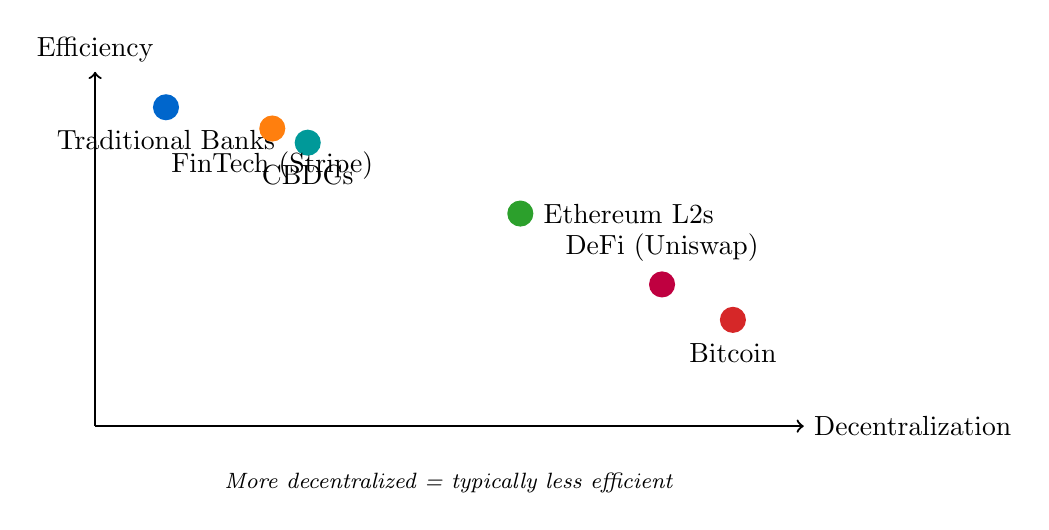
\begin{tikzpicture}[scale=0.9]
% Axis
\draw[thick, ->] (0,0) -- (10,0) node[right] {Decentralization};
\draw[thick, ->] (0,0) -- (0,5) node[above] {Efficiency};

% Points
\node[circle, fill=dfblue, minimum size=8pt, label=below:{Traditional Banks}] at (1,4.5) {};
\node[circle, fill=dfteal, minimum size=8pt, label=below:{CBDCs}] at (3,4) {};
\node[circle, fill=dforange, minimum size=8pt, label=below:{FinTech (Stripe)}] at (2.5,4.2) {};
\node[circle, fill=dfgreen, minimum size=8pt, label=right:{Ethereum L2s}] at (6,3) {};
\node[circle, fill=dfred, minimum size=8pt, label=below:{Bitcoin}] at (9,1.5) {};
\node[circle, fill=purple, minimum size=8pt, label=above:{DeFi (Uniswap)}] at (8,2) {};

% Labels
\node[font=\footnotesize] at (5,-0.8) {\textit{More decentralized = typically less efficient}};
\end{tikzpicture}
\end{center}

\textbf{Key insight:} Position on this spectrum is a \textit{choice}, not a flaw.
\end{frame}

% ---------------------------------------------------------------------
% Slide 12: Question 4 - RISKS
% ---------------------------------------------------------------------
\begin{frame}{Question 4: RISKS}
\begin{columns}[T]
\begin{column}{0.32\textwidth}
\textbf{Technical Risks:}
\begin{itemize}
\item Smart contract bugs
\item Oracle failures
\item Scalability limits
\item Key management
\item Dependency risks
\end{itemize}
\end{column}
\begin{column}{0.32\textwidth}
\textbf{Economic Risks:}
\begin{itemize}
\item Death spirals
\item Liquidity crises
\item Incentive misalignment
\item Bank runs
\item Market manipulation
\end{itemize}
\end{column}
\begin{column}{0.32\textwidth}
\textbf{Regulatory Risks:}
\begin{itemize}
\item Securities classification
\item Licensing requirements
\item Enforcement actions
\item Cross-border issues
\item Changing rules
\end{itemize}
\end{column}
\end{columns}

\vspace{0.5cm}
\textbf{Risk Assessment Questions:}
\begin{itemize}
\item What's the worst-case scenario?
\item Has something similar failed before? Why?
\item What's the attack surface?
\end{itemize}
\end{frame}

% ---------------------------------------------------------------------
% Slide 13: Risk Framework - Learning from Failures
% ---------------------------------------------------------------------
\begin{frame}{Risk Framework: Learning from Failures}
\begin{table}[h]
\centering
\footnotesize
\begin{tabular}{p{2.5cm}p{3cm}p{5cm}}
\toprule
\textbf{Failure} & \textbf{Risk Type} & \textbf{Lesson} \\
\midrule
Terra/Luna & Economic (death spiral) & Algorithmic pegs can fail catastrophically \\
\addlinespace
FTX & Governance (fraud) & Centralized custody requires oversight \\
\addlinespace
The DAO & Technical (reentrancy) & Smart contracts need rigorous audits \\
\addlinespace
Mt. Gox & Technical + Operational & Hot wallet security is critical \\
\addlinespace
Celsius & Economic + Governance & Yield sources must be sustainable \\
\bottomrule
\end{tabular}
\end{table}

\vspace{0.3cm}
\begin{exampleblock}{Pattern Recognition}
Most failures combine multiple risk types. Analyzing past failures helps identify future vulnerabilities.
\end{exampleblock}
\end{frame}

% ---------------------------------------------------------------------
% Slide 14: Question 5 - REGULATORY STATUS
% ---------------------------------------------------------------------
\begin{frame}{Question 5: REGULATORY STATUS}
\begin{block}{Key Sub-Questions}
\begin{itemize}
\item Is this a security, commodity, currency, or something else?
\item Which regulators have jurisdiction? (SEC, CFTC, FinCEN, state, international)
\item Has there been regulatory guidance or enforcement?
\item What's the compliance strategy? (Licensed, avoiding jurisdiction, fighting)
\item How might regulation evolve?
\end{itemize}
\end{block}

\vspace{0.3cm}
\textbf{Regulatory Classification Matters:}
\begin{table}[h]
\centering
\footnotesize
\begin{tabular}{ll}
\toprule
\textbf{If classified as...} & \textbf{Then...} \\
\midrule
Security & Must register with SEC or use exemptions \\
Commodity & CFTC oversight for derivatives \\
Money transmission & State licenses required \\
Banking product & OCC/Fed/FDIC oversight \\
\bottomrule
\end{tabular}
\end{table}
\end{frame}

% ---------------------------------------------------------------------
% Slide 15: Regulatory Spectrum
% ---------------------------------------------------------------------
\begin{frame}{The Regulatory Spectrum}
\begin{center}
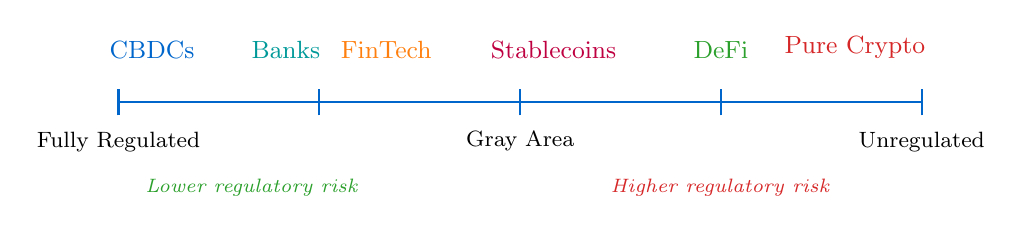
\begin{tikzpicture}[scale=0.85]
% Spectrum line
\draw[thick, dfblue] (0,0) -- (12,0);
\foreach \x in {0,3,6,9,12} {
    \draw[thick, dfblue] (\x,-0.2) -- (\x,0.2);
}

% Labels on spectrum
\node[below, font=\footnotesize] at (0,-0.3) {Fully Regulated};
\node[below, font=\footnotesize] at (6,-0.3) {Gray Area};
\node[below, font=\footnotesize] at (12,-0.3) {Unregulated};

% Innovations positioned
\node[above, font=\small, dfblue] at (0.5,0.5) {CBDCs};
\node[above, font=\small, dfteal] at (2.5,0.5) {Banks};
\node[above, font=\small, dforange] at (4,0.5) {FinTech};
\node[above, font=\small, purple] at (6.5,0.5) {Stablecoins};
\node[above, font=\small, dfgreen] at (9,0.5) {DeFi};
\node[above, font=\small, dfred] at (11,0.5) {Pure Crypto};

% Risk indication
\node[below, font=\scriptsize, dfred] at (9,-1) {\textit{Higher regulatory risk}};
\node[below, font=\scriptsize, dfgreen] at (2,-1) {\textit{Lower regulatory risk}};
\end{tikzpicture}
\end{center}

\vspace{0.5cm}
\begin{alertblock}{CBDC Advantage}
CBDCs have unique regulatory position: issued by the regulator itself, ensuring compliance by design.
\end{alertblock}
\end{frame}

% ---------------------------------------------------------------------
% Slide 16: Question 6 - WHO BENEFITS
% ---------------------------------------------------------------------
\begin{frame}{Question 6: WHO BENEFITS}
\begin{block}{Key Sub-Questions}
\begin{itemize}
\item Who captures the economic value? (Founders, investors, users, validators)
\item What are the fee structures and where do fees go?
\item Who bears the risks?
\item Are incentives aligned between stakeholders?
\item Who might be harmed? (Competitors, users of existing systems, society)
\end{itemize}
\end{block}

\vspace{0.3cm}
\begin{columns}[T]
\begin{column}{0.48\textwidth}
\textbf{Value Distribution Analysis:}
\begin{itemize}
\item Token allocation (team, investors, public)
\item Revenue model and fees
\item Governance rights
\end{itemize}
\end{column}
\begin{column}{0.48\textwidth}
\textbf{Red Flags:}
\begin{itemize}
\item Highly concentrated token ownership
\item Misaligned incentives
\item Users bear risk, insiders capture upside
\end{itemize}
\end{column}
\end{columns}
\end{frame}

% ---------------------------------------------------------------------
% Slide 17: Value Distribution Examples
% ---------------------------------------------------------------------
\begin{frame}{Value Distribution: Comparing Models}
\begin{table}[h]
\centering
\footnotesize
\begin{tabular}{p{2cm}p{3cm}p{3cm}p{3cm}}
\toprule
\textbf{Aspect} & \textbf{Stripe (FinTech)} & \textbf{Uniswap (DeFi)} & \textbf{CBDC} \\
\midrule
Value Capture & Shareholders & LPs + UNI holders & Central bank \\
\addlinespace
Fee Flow & Transaction fees to Stripe Inc. & 0.3\% to liquidity providers & Minimal/none \\
\addlinespace
Risk Bearer & Users + Stripe & Liquidity providers & Government \\
\addlinespace
Governance & Corporate board & Token voting (DAO) & Central bank \\
\bottomrule
\end{tabular}
\end{table}

\vspace{0.3cm}
\begin{exampleblock}{Insight}
Understanding value distribution reveals who has incentives to maintain and improve the system.
\end{exampleblock}
\end{frame}

% ---------------------------------------------------------------------
% Slide 18: The Six Dimensions Framework
% ---------------------------------------------------------------------
\begin{frame}{The Six Dimensions: Course-Aligned Evaluation}
\begin{center}
\textbf{Innovation Scorecard Dimensions}
\end{center}

\begin{table}[h]
\centering
\footnotesize
\begin{tabular}{clp{6cm}}
\toprule
\textbf{Day} & \textbf{Dimension} & \textbf{What It Measures} \\
\midrule
1 & Trust Architecture & How is trust established and maintained? \\
2 & Platform Dynamics & Network effects, ecosystem, switching costs \\
3 & Technical Soundness & Security, scalability, reliability \\
4 & Programmability & Smart contracts, composability, automation \\
5 & Risk Profile & Technical, economic, regulatory risks \\
6 & Future Potential & Growth trajectory, convergence potential \\
\bottomrule
\end{tabular}
\end{table}

\vspace{0.3cm}
\begin{block}{Scoring}
Each dimension: 5 criteria scored 1-5. Total: 30 evaluation points per innovation.
\end{block}
\end{frame}

% ---------------------------------------------------------------------
% Slide 19: Trust Architecture Dimension
% ---------------------------------------------------------------------
\begin{frame}{Dimension 1: Trust Architecture (Day 1)}
\textbf{How is trust established and maintained?}

\vspace{0.3cm}
\begin{columns}[T]
\begin{column}{0.32\textwidth}
\textbf{Centralized}
\begin{itemize}
\item Single trusted entity
\item Clear accountability
\item Single point of failure
\item Example: Stripe
\end{itemize}
\end{column}
\begin{column}{0.32\textwidth}
\textbf{Federated}
\begin{itemize}
\item Consortium of parties
\item Shared responsibility
\item Coordination required
\item Example: Digital Euro
\end{itemize}
\end{column}
\begin{column}{0.32\textwidth}
\textbf{Decentralized}
\begin{itemize}
\item Trust in code/algorithms
\item No single point of failure
\item Coordination via consensus
\item Example: Uniswap
\end{itemize}
\end{column}
\end{columns}

\vspace{0.5cm}
\begin{alertblock}{Key Insight}
No trust model is inherently superior---each suits different contexts and risk tolerances.
\end{alertblock}
\end{frame}

% ---------------------------------------------------------------------
% Slide 20: Platform Dynamics Dimension
% ---------------------------------------------------------------------
\begin{frame}{Dimension 2: Platform Dynamics (Day 2)}
\textbf{Criteria for Platform Assessment:}

\begin{enumerate}
\item \textbf{Network Effects}: Does value increase with more users?
\item \textbf{Developer Ecosystem}: APIs, tools, integrations available?
\item \textbf{User Experience}: Accessibility for target audience?
\item \textbf{Switching Costs}: How locked-in are users?
\item \textbf{Interoperability}: Works with other systems?
\end{enumerate}

\vspace{0.3cm}
\begin{exampleblock}{Platform Comparison}
\begin{itemize}
\item \textbf{Stripe}: Strong two-sided network effects, excellent developer ecosystem (5/5)
\item \textbf{Uniswap}: Liquidity network effects, low switching costs (4.2/5)
\item \textbf{Digital Euro}: Not yet launched, mandatory adoption likely (2.8/5)
\end{itemize}
\end{exampleblock}
\end{frame}

% ---------------------------------------------------------------------
% Slide 21: Technical Soundness Dimension
% ---------------------------------------------------------------------
\begin{frame}{Dimension 3: Technical Soundness (Day 3)}
\textbf{Criteria for Technical Assessment:}

\begin{enumerate}
\item \textbf{Security Architecture}: Audit history, vulnerability track record
\item \textbf{Scalability}: TPS, latency, cost per transaction
\item \textbf{Reliability}: Uptime, incident history
\item \textbf{Code Quality}: Documentation, testing, maintainability
\item \textbf{Team Expertise}: Track record, technical depth
\end{enumerate}

\vspace{0.3cm}
\begin{columns}[T]
\begin{column}{0.48\textwidth}
\textbf{Strong Signals:}
\begin{itemize}
\item Multiple independent audits
\item Open-source with active development
\item Formal verification where possible
\end{itemize}
\end{column}
\begin{column}{0.48\textwidth}
\textbf{Warning Signs:}
\begin{itemize}
\item No audits or single audit
\item Closed source or abandoned
\item Complex with no clear purpose
\end{itemize}
\end{column}
\end{columns}
\end{frame}

% ---------------------------------------------------------------------
% Slide 22: Programmability Dimension
% ---------------------------------------------------------------------
\begin{frame}{Dimension 4: Programmability (Day 4)}
\textbf{Criteria for Programmability Assessment:}

\begin{enumerate}
\item \textbf{Smart Contract Support}: Native or none?
\item \textbf{Composability}: Can combine with other protocols?
\item \textbf{Automation}: Programmable conditions and triggers?
\item \textbf{API/SDK Quality}: Developer tools available?
\item \textbf{Extensibility}: Can third parties build on it?
\end{enumerate}

\vspace{0.3cm}
\begin{table}[h]
\centering
\footnotesize
\begin{tabular}{lccc}
\toprule
\textbf{Feature} & \textbf{Stripe} & \textbf{Uniswap} & \textbf{Digital Euro} \\
\midrule
Smart Contracts & Limited & Full (Turing-complete) & Minimal \\
Composability & API-based & ``Money Legos'' & Restricted \\
Score & 3.8/5 & 5.0/5 & 3.0/5 \\
\bottomrule
\end{tabular}
\end{table}

\textbf{Key tension:} Higher programmability often means higher regulatory uncertainty.
\end{frame}

% ---------------------------------------------------------------------
% Slide 23: Risk Profile Dimension
% ---------------------------------------------------------------------
\begin{frame}{Dimension 5: Risk Profile (Day 5)}
\textbf{Criteria for Risk Assessment:}

\begin{enumerate}
\item \textbf{Regulatory Risk}: Clarity of legal status
\item \textbf{Counterparty Risk}: Dependence on specific parties
\item \textbf{Smart Contract Risk}: Bug and exploit exposure
\item \textbf{Market Risk}: Price volatility impact
\item \textbf{Operational Risk}: Team, governance, continuity
\end{enumerate}

\vspace{0.3cm}
\begin{alertblock}{Impermanent Loss Example}
Uniswap liquidity providers face ``impermanent loss'' when token prices diverge---an economic risk unique to AMMs that becomes permanent when liquidity is withdrawn.
\end{alertblock}

\textbf{Pattern:} Higher programmability and decentralization often correlate with higher regulatory risk.
\end{frame}

% ---------------------------------------------------------------------
% Slide 24: Future Potential Dimension
% ---------------------------------------------------------------------
\begin{frame}{Dimension 6: Future Potential (Day 6)}
\textbf{Criteria for Future Assessment:}

\begin{enumerate}
\item \textbf{Market Growth}: TAM expansion trajectory
\item \textbf{Technology Roadmap}: Clear evolution path?
\item \textbf{Competitive Position}: Defensible advantages?
\item \textbf{Convergence Potential}: Integration with other paradigms?
\item \textbf{Adaptability}: Can pivot to regulatory/market changes?
\end{enumerate}

\vspace{0.3cm}
\begin{exampleblock}{Innovation Trajectories}
\begin{itemize}
\item \textbf{Uniswap}: V3 concentrated liquidity (100x capital efficiency), V4 hooks
\item \textbf{Stripe}: Expanding to crypto, embedded finance, global coverage
\item \textbf{Digital Euro}: Pilot phase, 2025-2027 potential launch
\end{itemize}
\end{exampleblock}
\end{frame}

% ---------------------------------------------------------------------
% Slide 25: Hands-On Exercise Introduction (NB14)
% ---------------------------------------------------------------------
\begin{frame}{Hands-On Exercise: Innovation Scorecard (NB14)}
\textbf{What you'll do in the notebook:}
\begin{enumerate}
\item Select a digital finance innovation to evaluate
\item Work through each of the six questions systematically
\item Score the innovation on key dimensions
\item Visualize your analysis (radar chart)
\item Compare with classmates' analyses
\end{enumerate}

\vspace{0.3cm}
\begin{block}{Suggested Innovations to Analyze}
\begin{multicols}{2}
\begin{itemize}
\item Real-world asset tokenization
\item Decentralized identity
\item AI-managed portfolios
\item Central Bank Digital Currencies
\item Prediction markets
\item Decentralized insurance
\item Tokenized treasuries
\item Cross-chain bridges
\end{itemize}
\end{multicols}
\end{block}

\bottomnote{Notebook: NB14\_Innovation\_Scorecard.ipynb}
\end{frame}

% ---------------------------------------------------------------------
% Slide 26: Exercise Walkthrough
% ---------------------------------------------------------------------
\begin{frame}{Exercise Walkthrough: Scorecard Methodology}
\textbf{Step-by-Step Process:}

\begin{enumerate}
\item \textbf{Research Phase} (10 min)
    \begin{itemize}
    \item Gather information on your chosen innovation
    \item Identify the problem, mechanism, and stakeholders
    \end{itemize}

\item \textbf{Scoring Phase} (15 min)
    \begin{itemize}
    \item Rate each of 30 criteria (6 dimensions $\times$ 5 criteria)
    \item Use 1-5 scale: 1=Poor, 3=Average, 5=Excellent
    \end{itemize}

\item \textbf{Visualization Phase} (5 min)
    \begin{itemize}
    \item Generate radar chart comparing dimensions
    \item Identify strengths and weaknesses
    \end{itemize}

\item \textbf{Reflection Phase} (10 min)
    \begin{itemize}
    \item Compare with peers' analyses
    \item Discuss scoring differences and rationale
    \end{itemize}
\end{enumerate}
\end{frame}

% ---------------------------------------------------------------------
% Slide 27: Application - Stablecoins Analysis
% ---------------------------------------------------------------------
\begin{frame}{Applying the Framework: Stablecoins}
\begin{center}
\textbf{Quick Scorecard: Stablecoins}
\end{center}

\begin{table}[h]
\centering
\footnotesize
\begin{tabular}{lp{9cm}}
\toprule
\textbf{Question} & \textbf{Analysis} \\
\midrule
PROBLEM & Dollar-denominated value transfer on blockchain; hedging crypto volatility \\
MECHANISM & Varies: fiat-backed (USDC), crypto-backed (DAI), algorithmic (failed: UST) \\
TRADEOFFS & Centralized (USDC) = more stable but censorable; Decentralized (DAI) = more complex \\
RISKS & Reserve quality, depegs, regulatory crackdown, bank runs \\
REGULATORY & Money transmission + potential securities issues; evolving globally \\
WHO BENEFITS & Issuers (interest on reserves), traders (liquidity), DeFi (composability) \\
\bottomrule
\end{tabular}
\end{table}
\end{frame}

% ---------------------------------------------------------------------
% Slide 28: Application - Comparing Three Paradigms
% ---------------------------------------------------------------------
\begin{frame}{Comparing Three Paradigms}
\begin{center}
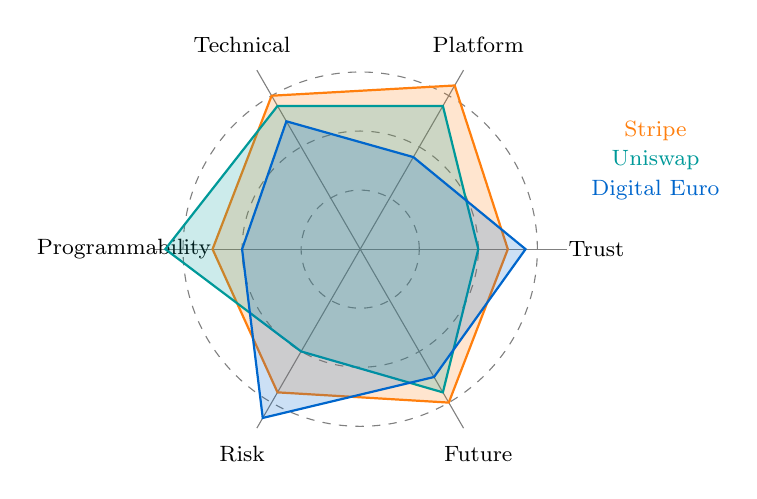
\begin{tikzpicture}[scale=0.75]
% Radar chart axes
\foreach \i/\label in {0/Trust, 60/Platform, 120/Technical, 180/Programmability, 240/Risk, 300/Future} {
    \draw[gray, thin] (0,0) -- (\i:3.5);
    \node[font=\footnotesize] at (\i:4) {\label};
}
% Circles
\foreach \r in {1,2,3} {
    \draw[gray, thin, dashed] (0,0) circle (\r);
}

% Stripe (orange)
\draw[dforange, thick, fill=dforange, fill opacity=0.2]
    (0:2.5) -- (60:3.2) -- (120:3) -- (180:2.5) -- (240:2.8) -- (300:3) -- cycle;

% Uniswap (teal)
\draw[dfteal, thick, fill=dfteal, fill opacity=0.2]
    (0:2) -- (60:2.8) -- (120:2.8) -- (180:3.3) -- (240:2) -- (300:2.8) -- cycle;

% Digital Euro (blue)
\draw[dfblue, thick, fill=dfblue, fill opacity=0.2]
    (0:2.8) -- (60:1.8) -- (120:2.5) -- (180:2) -- (240:3.3) -- (300:2.5) -- cycle;

% Legend
\node[font=\footnotesize, dforange] at (5,2) {Stripe};
\node[font=\footnotesize, dfteal] at (5,1.5) {Uniswap};
\node[font=\footnotesize, dfblue] at (5,1) {Digital Euro};
\end{tikzpicture}
\end{center}

\textbf{Key insight:} Each paradigm optimizes for different dimensions---there is no universal ``best.''
\end{frame}

% ---------------------------------------------------------------------
% Slide 29: Discussion - Trade-off Patterns
% ---------------------------------------------------------------------
\begin{frame}{Discussion: Trade-off Patterns}
\textbf{Emerging Pattern: Programmability vs. Regulatory Clarity}

\vspace{0.3cm}
\begin{center}
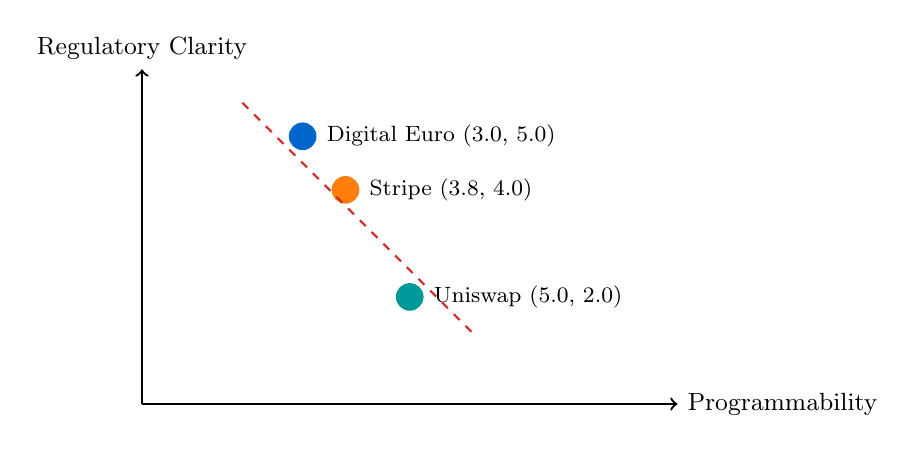
\begin{tikzpicture}[scale=0.85]
% Axes
\draw[thick, ->] (0,0) -- (8,0) node[right, font=\small] {Programmability};
\draw[thick, ->] (0,0) -- (0,5) node[above, font=\small] {Regulatory Clarity};

% Points
\node[circle, fill=dfblue, minimum size=10pt, label=right:{\footnotesize Digital Euro (3.0, 5.0)}] at (2.4,4) {};
\node[circle, fill=dforange, minimum size=10pt, label=right:{\footnotesize Stripe (3.8, 4.0)}] at (3.04,3.2) {};
\node[circle, fill=dfteal, minimum size=10pt, label=right:{\footnotesize Uniswap (5.0, 2.0)}] at (4,1.6) {};

% Trend line
\draw[dashed, dfred, thick] (1.5,4.5) -- (5,1);
\end{tikzpicture}
\end{center}

\begin{alertblock}{Discussion Question}
Is this tradeoff inevitable, or can future innovations achieve both high programmability AND regulatory clarity?
\end{alertblock}
\end{frame}

% ---------------------------------------------------------------------
% Slide 30: Synthesis - The Four Lenses
% ---------------------------------------------------------------------
\begin{frame}{Synthesis: The Lenses We've Developed}
\begin{center}
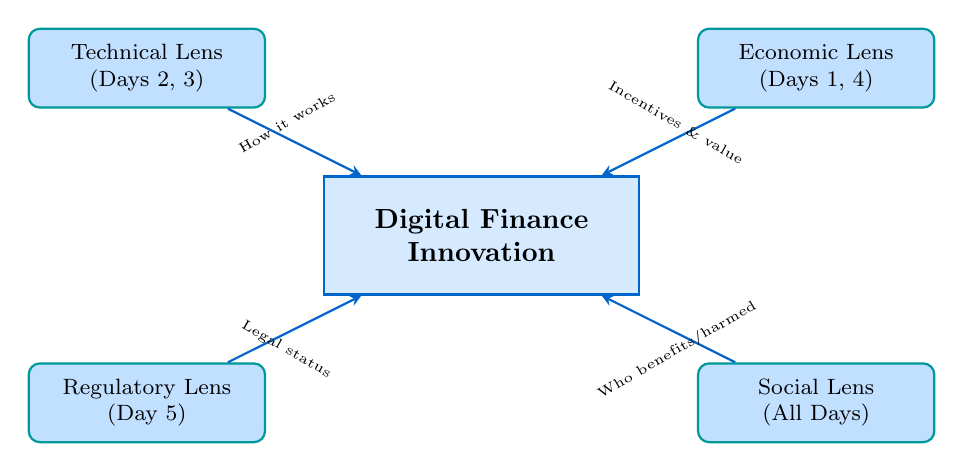
\begin{tikzpicture}[scale=0.85]
% Central node
\node[process, minimum width=4cm, minimum height=1.5cm, font=\bfseries, align=center] (center) at (0,0) {Digital Finance\\Innovation};

% Four lenses
\node[blockchain, minimum width=3cm, font=\footnotesize, align=center] (tech) at (-5,2.5) {Technical Lens\\(Days 2, 3)};
\node[blockchain, minimum width=3cm, font=\footnotesize, align=center] (econ) at (5,2.5) {Economic Lens\\(Days 1, 4)};
\node[blockchain, minimum width=3cm, font=\footnotesize, align=center] (reg) at (-5,-2.5) {Regulatory Lens\\(Day 5)};
\node[blockchain, minimum width=3cm, font=\footnotesize, align=center] (social) at (5,-2.5) {Social Lens\\(All Days)};

% Arrows
\draw[arrow] (tech) -- (center);
\draw[arrow] (econ) -- (center);
\draw[arrow] (reg) -- (center);
\draw[arrow] (social) -- (center);

% Labels on arrows
\node[font=\tiny, above, rotate=30] at (-2.8,1.5) {How it works};
\node[font=\tiny, above, rotate=-30] at (2.8,1.5) {Incentives \& value};
\node[font=\tiny, below, rotate=-30] at (-2.8,-1.5) {Legal status};
\node[font=\tiny, below, rotate=30] at (2.8,-1.5) {Who benefits/harmed};
\end{tikzpicture}
\end{center}

\textbf{Complete analysis requires all four lenses.}
\end{frame}

% ---------------------------------------------------------------------
% Slide 31: Executive Summary
% ---------------------------------------------------------------------
\begin{frame}{Executive Summary}
\begin{block}{The Innovation Scorecard Framework}
\textbf{Six Questions} to ask about ANY digital finance innovation:
\begin{enumerate}
\item PROBLEM: What real problem does this solve?
\item MECHANISM: How does it actually work?
\item TRADEOFFS: What was sacrificed for what gain?
\item RISKS: What could go wrong?
\item REGULATORY: Where does it fit legally?
\item WHO BENEFITS: Who captures value vs. bears costs?
\end{enumerate}
\end{block}

\begin{alertblock}{Key Principles}
\begin{itemize}
\item \textbf{No perfect solution}: Every innovation makes trade-offs
\item \textbf{Context matters}: Different use cases favor different models
\item \textbf{Focus on durables}: Principles outlast specific implementations
\end{itemize}
\end{alertblock}
\end{frame}

% ---------------------------------------------------------------------
% Slide 32: Concept Map
% ---------------------------------------------------------------------
\begin{frame}{Concept Map: Building Your Worldview}
\begin{center}
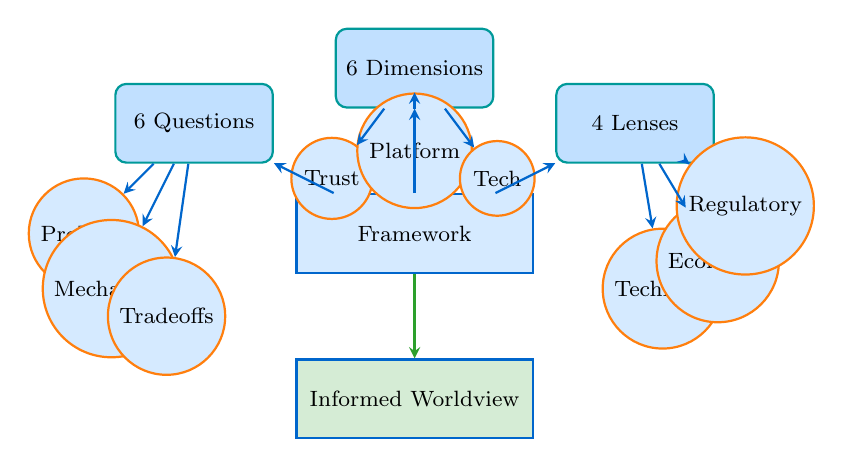
\begin{tikzpicture}[scale=0.7, every node/.style={font=\footnotesize}]
% Central concept
\node[process, minimum width=3cm] (fw) at (0,0) {Framework};

% Level 1
\node[blockchain, minimum width=2cm] (q) at (-4,2) {6 Questions};
\node[blockchain, minimum width=2cm] (d) at (0,3) {6 Dimensions};
\node[blockchain, minimum width=2cm] (l) at (4,2) {4 Lenses};

% Level 2 - Questions
\node[transaction, minimum size=0.6cm] (q1) at (-6,0) {Problem};
\node[transaction, minimum size=0.6cm] (q2) at (-5.5,-1) {Mechanism};
\node[transaction, minimum size=0.6cm] (q3) at (-4.5,-1.5) {Tradeoffs};

% Level 2 - Dimensions
\node[transaction, minimum size=0.6cm] (d1) at (-1.5,1) {Trust};
\node[transaction, minimum size=0.6cm] (d2) at (0,1.5) {Platform};
\node[transaction, minimum size=0.6cm] (d3) at (1.5,1) {Tech};

% Level 2 - Lenses
\node[transaction, minimum size=0.6cm] (l1) at (4.5,-1) {Technical};
\node[transaction, minimum size=0.6cm] (l2) at (5.5,-0.5) {Economic};
\node[transaction, minimum size=0.6cm] (l3) at (6,0.5) {Regulatory};

% Connections
\draw[arrow] (fw) -- (q);
\draw[arrow] (fw) -- (d);
\draw[arrow] (fw) -- (l);
\draw[arrow] (q) -- (q1);
\draw[arrow] (q) -- (q2);
\draw[arrow] (q) -- (q3);
\draw[arrow] (d) -- (d1);
\draw[arrow] (d) -- (d2);
\draw[arrow] (d) -- (d3);
\draw[arrow] (l) -- (l1);
\draw[arrow] (l) -- (l2);
\draw[arrow] (l) -- (l3);

% Output
\node[process, minimum width=3cm, fill=dfgreen!20] (out) at (0,-3) {Informed Worldview};
\draw[arrow, thick, dfgreen] (fw) -- (out);
\end{tikzpicture}
\end{center}
\end{frame}

% ---------------------------------------------------------------------
% Slide 33: Key Terms (Part 1)
% ---------------------------------------------------------------------
\begin{frame}{Key Terms (1/2)}
\begin{description}
\item[Innovation Scorecard] Systematic framework for evaluating digital finance innovations across six dimensions

\item[Trust Architecture] How an innovation establishes and maintains trust (centralized, federated, or decentralized)

\item[Composability] Ability of protocols to combine like ``money legos''---building complex products from simple primitives

\item[Impermanent Loss] Economic risk for AMM liquidity providers when token prices diverge from initial ratio

\item[Constant Product Formula] $x \times y = k$: Mathematical relationship maintaining AMM liquidity pool balance

\item[Platform Dynamics] Network effects, ecosystem strength, and switching costs that determine competitive position
\end{description}
\end{frame}

% ---------------------------------------------------------------------
% Slide 34: Key Terms (Part 2)
% ---------------------------------------------------------------------
\begin{frame}{Key Terms (2/2)}
\begin{description}
\item[Technical Soundness] Assessment of security, scalability, reliability, code quality, and team expertise

\item[Programmability] Degree to which an innovation supports smart contracts, automation, and third-party development

\item[Risk Profile] Comprehensive assessment of technical, economic, regulatory, and operational risks

\item[Concentrated Liquidity] Uniswap V3 innovation allowing LPs to focus capital in specific price ranges (up to 100x efficiency)

\item[Bank Disintermediation] Risk that CBDCs cause deposit flight from commercial banks, addressed via holding limits

\item[Regulatory Arbitrage] Strategy of operating in jurisdictions with favorable or unclear regulations
\end{description}
\end{frame}

% ---------------------------------------------------------------------
% Slide 35: Common Misconceptions
% ---------------------------------------------------------------------
\begin{frame}{Common Misconceptions}
\begin{columns}[T]
\begin{column}{0.48\textwidth}
\textbf{Misconception:}
\begin{itemize}
\item ``Decentralization is always better''
\item ``Higher scores mean better investments''
\item ``FinTech and DeFi are in competition''
\item ``Regulation kills innovation''
\item ``Technical security equals safety''
\end{itemize}
\end{column}
\begin{column}{0.48\textwidth}
\textbf{Reality:}
\begin{itemize}
\item Optimal trust model depends on use case
\item Context determines which tradeoffs matter
\item Convergence creates hybrid solutions
\item Smart regulation enables sustainable growth
\item Economic and governance risks can be larger
\end{itemize}
\end{column}
\end{columns}

\vspace{0.5cm}
\begin{alertblock}{Critical Thinking}
The framework helps you ask better questions, not give you definitive answers. Your judgment, informed by context, remains essential.
\end{alertblock}
\end{frame}

% ---------------------------------------------------------------------
% Slide 36: Self-Assessment Question 1
% ---------------------------------------------------------------------
\begin{frame}{Self-Assessment Question 1}
\begin{block}{Question}
What is the primary purpose of the Innovation Scorecard framework presented in NB14?
\end{block}

\vspace{0.3cm}
\begin{enumerate}[A.]
\item To rank cryptocurrencies by market capitalization
\item To systematically evaluate digital finance innovations across multiple dimensions
\item To predict stock prices of fintech companies
\item To calculate the profitability of DeFi protocols
\end{enumerate}

\vspace{0.5cm}
\pause
\begin{exampleblock}{Answer: B}
The Innovation Scorecard evaluates innovations across six dimensions: trust architecture, platform dynamics, technical soundness, programmability, risk profile, and future potential. It provides systematic assessment rather than focusing on a single metric.
\end{exampleblock}
\end{frame}

% ---------------------------------------------------------------------
% Slide 37: Self-Assessment Questions 2-3
% ---------------------------------------------------------------------
\begin{frame}{Self-Assessment Questions 2-3}
\begin{block}{Question 2}
What is the primary regulatory advantage of CBDCs like the Digital Euro?
\end{block}
\textbf{Answer:} They are issued by the regulator itself, ensuring compliance by design (5/5 regulatory score).

\vspace{0.5cm}
\begin{block}{Question 3}
Why does the Digital Euro propose holding limits?
\end{block}
\textbf{Answer:} To prevent bank disintermediation and systemic risk. Unlimited CBDC holdings could cause deposits to migrate from commercial banks, destabilizing the banking system that relies on deposits for lending.

\vspace{0.3cm}
\begin{alertblock}{Key Insight}
These questions illustrate how regulatory design (Question 2) and economic considerations (Question 3) interact in real-world innovation decisions.
\end{alertblock}
\end{frame}

% ---------------------------------------------------------------------
% Slide 38: What's Next
% ---------------------------------------------------------------------
\begin{frame}{What's Next: Topic 6.4 - What's Next?}
\textbf{Preview of T6.4: What's Next in Digital Finance}

\vspace{0.3cm}
\begin{columns}[T]
\begin{column}{0.48\textwidth}
\textbf{Emerging Trends:}
\begin{itemize}
\item AI-native financial services
\item Real-world asset tokenization at scale
\item CBDC interoperability
\item Privacy-preserving compliance
\item Embedded finance everywhere
\end{itemize}
\end{column}
\begin{column}{0.48\textwidth}
\textbf{Your Toolkit:}
\begin{itemize}
\item Apply the Innovation Scorecard
\item Use the four analytical lenses
\item Focus on durable principles
\item Recognize patterns across innovations
\item Think critically about trade-offs
\end{itemize}
\end{column}
\end{columns}

\vspace{0.5cm}
\begin{block}{Preparation}
Bring your completed Innovation Scorecard analysis from NB14 to discuss emerging innovations using your new framework.
\end{block}
\end{frame}

% ---------------------------------------------------------------------
% Slide 39: Resources
% ---------------------------------------------------------------------
\begin{frame}{Resources}
\textbf{Course Materials:}
\begin{itemize}
\item NB14: Innovation Scorecard (hands-on exercise)
\item Day 1-6 slide decks (reference for each dimension)
\end{itemize}

\vspace{0.3cm}
\textbf{Further Reading:}
\begin{itemize}
\item Nakamoto, S. (2008). ``Bitcoin: A Peer-to-Peer Electronic Cash System''
\item Buterin, V. (2014). ``Ethereum Whitepaper''
\item Adams, H. et al. (2020). ``Uniswap v2 Core''
\item ECB (2023). ``Digital Euro: Progress Report''
\item BIS (2024). ``Annual Economic Report'' - Chapter on Digital Currencies
\end{itemize}

\vspace{0.3cm}
\textbf{Tools:}
\begin{itemize}
\item DeFi Llama (defillama.com) - Protocol analytics
\item L2Beat (l2beat.com) - Layer 2 comparison
\item Token Terminal - Financial metrics for protocols
\end{itemize}
\end{frame}

% ---------------------------------------------------------------------
% Slide 40: Questions?
% ---------------------------------------------------------------------
\begin{frame}{Questions?}
\begin{center}
\vspace{1cm}
{\Large \textbf{Questions and Discussion}}

\vspace{1cm}
\textbf{Topic 6.3: Building Your Digital Finance Worldview}

\vspace{0.5cm}
A Framework for Evaluating Innovation

\vspace{1cm}
\begin{block}{Key Takeaway}
The goal is not to memorize facts that will change, but to develop a way of thinking that helps you evaluate \textit{any} digital finance innovation---today and in the future.
\end{block}

\vspace{0.5cm}
\textit{Next: Topic 6.4 - What's Next in Digital Finance}
\end{center}
\end{frame}

\end{document}
